\chapter{Methods}
\label{sec:methods}
In this section, the so-called $\Lambda \Omega$ systems are introduced. In addition, a special class of $\Lambda \Omega$ systems, the $\Lambda \Omega_{2}$ system, is presented and degeneracy is characterized on this particular system. We also establish how $\Lambda \Omega_{2}$ systems are interconnected in order to form $\Lambda \Omega_{2}$ networks, where the degeneracy problem will be studied.

Important concepts such as attribute level sets or total-degeneracy are also defined in this section.   

\section{$\Lambda \Omega$ Systems}
$\Lambda \Omega$ systems are simple oscillatory systems. Equations describing $\Lambda \Omega$ systems have the general form

\begin{equation}
    \frac{dx}{dt} = \Lambda(r)x-\Omega(r)y
    \label{e1}
\end{equation}
\begin{equation}
    \frac{dy}{dt} = \Omega(r)x+\Lambda(r)y
    \label{e2}
\end{equation}
with
\begin{equation}
r^{2}=x^{2}+y^{2}
\label{e3}
\end{equation}

where x and y are state variables and t is time. $\Lambda$ and $\Omega$ are real functions of single variable. The system is linear only if functions $\Lambda$ and $\Omega$ are constants. Otherwise, $\Lambda \Omega$ systems are a class of non-linear system of ordinary differential equations.

They have been extensively used as the kinetics in the study of wave phenomena in reaction diffusion models, \cite{Kopell1973}. These class of reaction diffusion systems have the advantage that explicit analytic solutions can be written down. However, we use the so-called $\Lambda \Omega$ systems as a class of non-trivial mathematical oscillators.

In \cite{LeonGlass2001}, $\Lambda \Omega$ systems are proposed as simple models useful to study synchronization of physiological oscillators, for example in populations of cells that generate the heart beat or gamma and beta rhythms in the brain.
They have also been used as mathematical models for central pattern generators \cite{Murray2002}, neural networks which exhibit rhythmic oscillations and do not require any external input to generate them.

It is convenient to study these systems in polar coordinates in the state space. A change of coordinates, from Cartesian to Polar

\begin{equation}
    x = r\cos(\theta) \hspace{0.5cm} \text{and} \hspace{0.5cm} y = r\sin(\theta)
    \label{e4}
\end{equation}

transforms system (\ref{e1})-(\ref{e2}) into

\begin{equation}
    \frac{dr}{dt} = r\Lambda(r)
    \label{e5}
\end{equation}
\begin{equation}
    \frac{d\theta}{dt} = \Omega(r)
    \label{e6}
\end{equation}

This form allows for the computation of the redius of the circular limit circle(s) as the solution(s) of

\begin{equation}
    \Lambda(\bar{r}) = 0
    \label{e7}
\end{equation}

We notice that a limit circle of radius $\bar{r}$ is stable if and only if $\Lambda(\bar{r})<0$. More stability details depend on functions $\Lambda(r)$ and $\Omega(r)$.

\subsection{$\Lambda \Omega_{2}$ Systems}
$\Lambda \Omega$ systems of order two ($\Lambda \Omega_{2}$) correspond to the following quadratic choices for $\Lambda(r)$ and $\Omega(r)$

\begin{equation}
    \Lambda(r) = \lambda - br^{2} \hspace{0.5cm} \text{and} \hspace{0.5cm} \Omega(r) = \omega + ar^{2}
    \label{e8}
\end{equation}

These functions belong to a specific class of $\Lambda$ and $\Omega$ functions introduced in \cite{Blowey2005,Garvie2005}, where they considered arbitrary power of the radius and performed an exhaustive mathematical and numerical analysis of these $\Lambda \Omega$ type oscillatory reaction diffusion equations.

Therefore, $\Lambda \Omega$ systems of order two ($\Lambda \Omega_{2}$), are given by Eqs. (\ref{e1}-\ref{e2}), when functions $\Lambda$ and $\Omega$ take the form in Eq. (\ref{e8}).

$\Lambda \Omega_{2}$ systems have a set of four parameters: $\lambda$, $b$, $\omega$ and a. As we study the degeneracy problem on networks composed by units of $\Lambda \Omega_{2}$ systems, we will refer to these parameters as the intrinsic parameters, in order to distinguish between connectivity parameters of the network and parameters from each $\Lambda \Omega_{2}$ system in the network.

$\Lambda \Omega_{2}$ systems have a single limit circle for 

\begin{equation}
    \bar{r} = \sqrt{\frac{\lambda}{b}}
     \label{e9}
\end{equation}

if $\lambda/b>0$ which is stable if and only if $b>0$. Therefore, only when parameters $\lambda$ and $b$ are both positive the system show sustained oscillations. Moreover, as parameter $\lambda$ becomes positive, the stable fixed point $(\bar{x},\bar{y})$ becomes unstable and the system undergoes a supercritical Hopf bifurcation.

Fig. (\ref{photo7}) shows the nullclines and the trajectory for a representative solution to the $\Lambda \Omega_{2}$ system. It is also shown the sinusoidal-like solutions of the state variables as a function of time.

\begin{figure}[h]
  \begin{minipage}{0.45\linewidth}
  \begin{center}
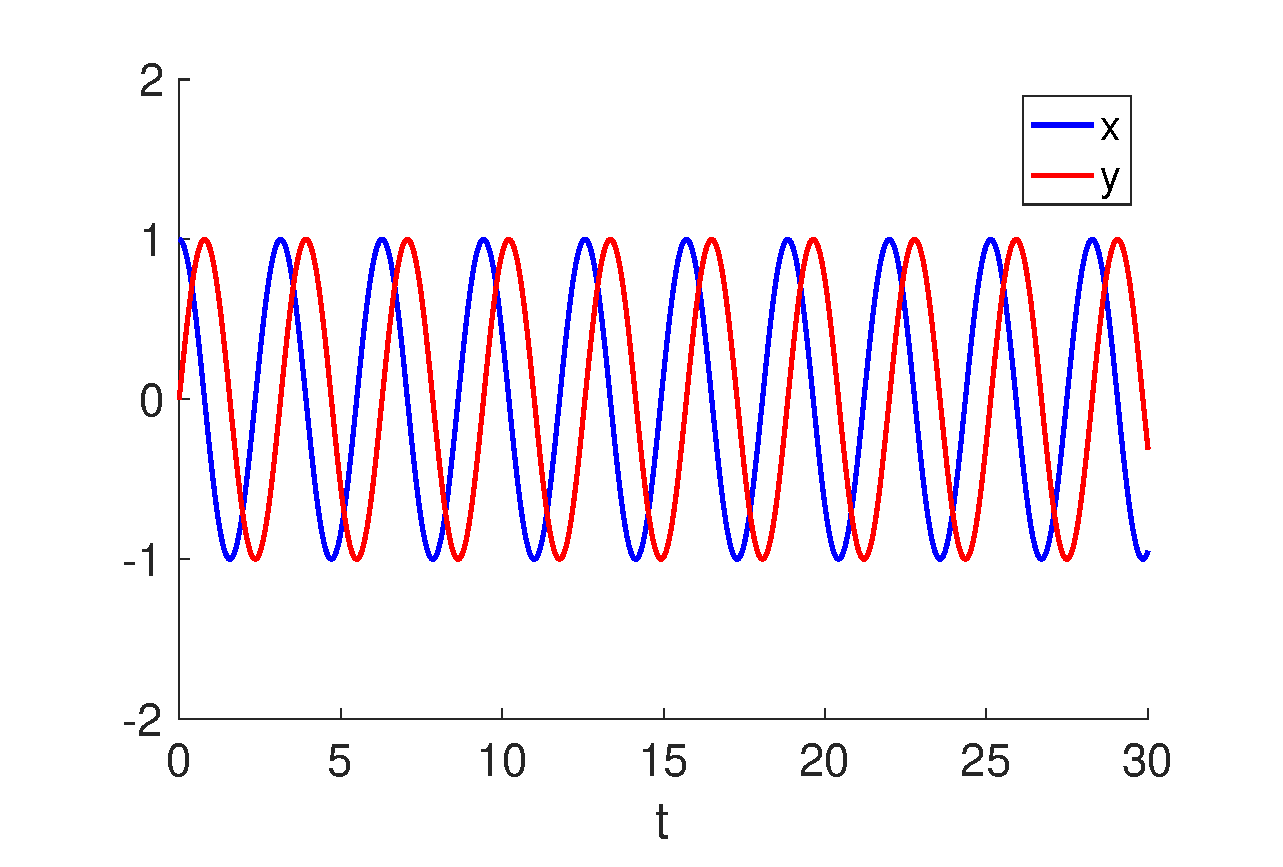
\includegraphics[width=1\linewidth]{Images/photo7_1.eps}
\end{center}
  \end{minipage} 
  \begin{minipage}{0.45\linewidth}
  \begin{center}
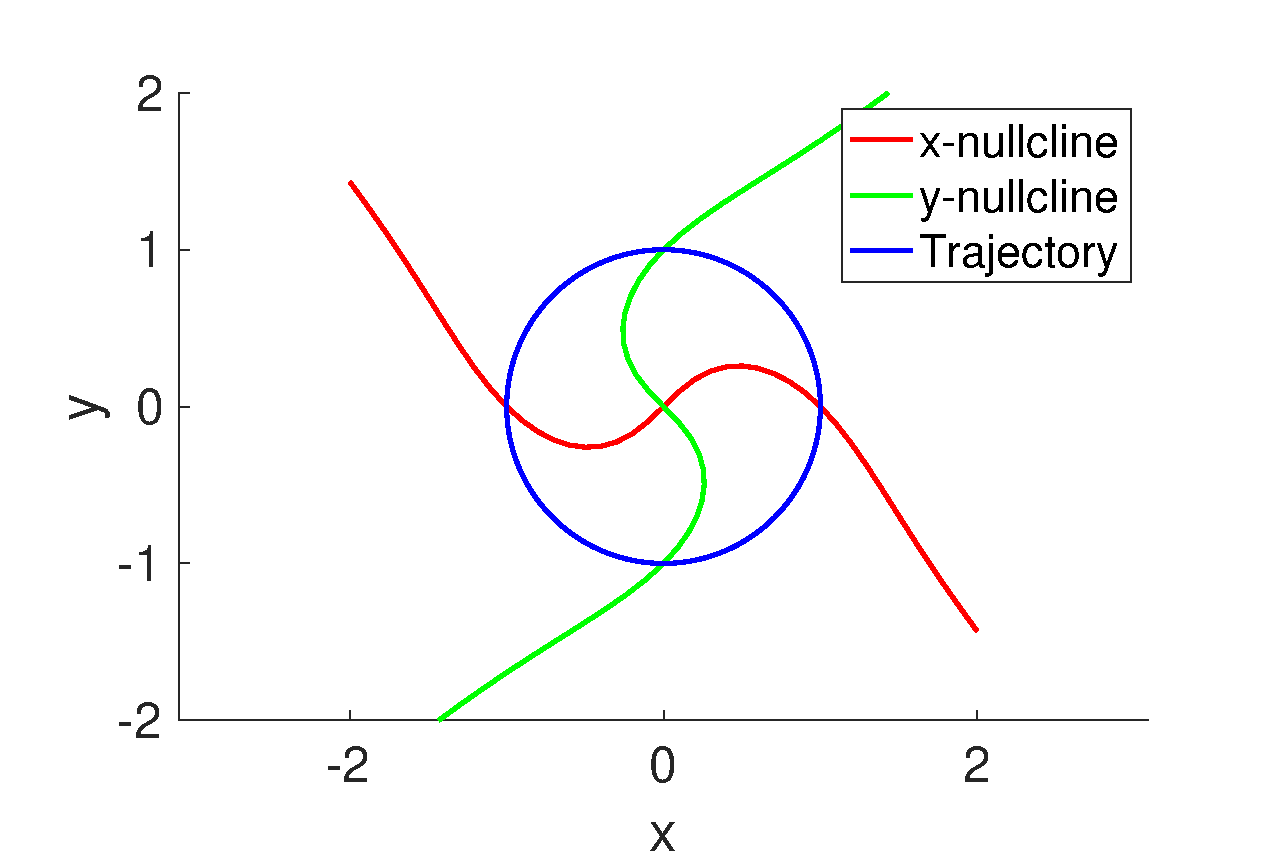
\includegraphics[width=1\linewidth]{Images/photo7_2.eps}
\end{center}
  \end{minipage} 
  \caption{\textbf{Dynamics of the $\Lambda \Omega_{2}$ systems.} Left: traces (curves of x and y as a function of t). Right: phase-plane diagram. The x- and y- nullclines are the set of points in the x-y plane that make $dx/dt=0$ and $dy/dt=0$ respectively. Parameter values: $\lambda = 1$, $b=1$, $a = 1$ and $\omega = 1$.}
  \label{photo7}
\end{figure}

Since we are interested in $\Lambda \Omega_{2}$ systems as mathematical oscillators we focus on the case when $\Lambda \Omega_{2}$ systems show a stable limit circle, towards which solutions converge in the limit of $t\rightarrow \infty$. We characterize the stationary oscillatory solutions by two attributes of the oscillatory pattern: the amplitude and frequency.

Simple theoretical oscillatory models, such as $\Lambda \Omega_{2}$ systems, are useful to study qualitative aspects of real physiological systems, from which they tend to be realistic simplifications. In this work, we consider $\Lambda \Omega_{2}$ systems as simplified models that simulate the behaviour of a neuronal cell. However, these $\Lambda \Omega_{2}$ models are too oversimplified to accurately represent a realistic neuron. Nonetheless, we shall consider the $\Lambda \Omega_{2}$ system as a toy model which would represent the behaviour of an hypothetical neuron.

In this respect, we consider variable x in Eq. (\ref{e4}) as the corresponding variable representing the voltage of an hypothetical cell modelled by a $\Lambda \Omega_{2}$ system. Furthermore, all attributes considered will characterized the oscillatory pattern of the cell voltage, i.e., variable x in the $\Lambda \Omega_{2}$ system.

\section{$\Lambda \Omega_{2}$ Networks}
The general form of the linear connectivity networks we consider is

\begin{equation}
    \frac{dx_{k}}{dt} = \Lambda_{k}(r_{k})x_{k} - \Omega_{k}(r_{k})y_{k} - \sum_{j=1}^{N}\alpha_{k,j}x_{j}
    \label{e10}
\end{equation}
\begin{equation}
    \frac{dy_{k}}{dt} = \Omega_{k}(r_{k})x_{k} + \Lambda_{k}(r_{k})y_{k}
    \label{e11}
\end{equation}

where

\begin{equation}
r_{k}^{2}=x_{k}^{2}+y_{k}^{2}
\label{e12}
\end{equation}

and $A=\{\alpha_{k,j}\}$ is the connectivity matrix. We shall call $\alpha_{k,k}$ self-connectivity parameters and $\alpha_{k,j}$ ($k \neq j$) cross-connectivity parameters.

$\Lambda \Omega_{2}$ networks and then given by Eqs. (\ref{e10})-(\ref{e11}) taking 

\begin{equation}
    \Lambda_{k}(r_{k}) = \lambda_{k} - b_{k}r_{k}^{2} \hspace{0.5cm} \text{and} \hspace{0.5cm} \Omega_{k}(r_{k}) = \omega_{k} + a_{k}r_{k}^{2}
    \label{e13}
\end{equation}

In this work, we consider $\Lambda \Omega_{2}$ networks composed by one and two units of $\Lambda \Omega_{2}$ systems. As we consider that $\Lambda \Omega_{2}$ systems represent the behaviour of an hypothetical neuronal cell, we shall refer to these networks as the self-connected cell and the two-cell network. The goal of the project is to characterize degeneracy in these two simple networks.

Based on the intrinsic parameters of the cells, we distinguish three different types of networks: homogeneous networks (cells are identical), type-I heterogeneous networks (cells belong to the same individual amplitude and frequency LS) and type-II heterogeneous networks (cells belong to different frequency and/or amplitude LS).

\section{Degeneracy and attribute level sets}
Degeneracy, in a model which involve parameters, refers to the situation where multiple sets of parameter values can produce the same observable output or attribute. In such a model, attribute level sets are defined as the set of points on parameter space for which a given attribute is constant.

In this work, we compute several attribute level sets in $\Lambda \Omega_{2}$ networks. We focus our analysis on 1 and 2-dimensional attribute level sets, embedded in 2,3 or 4-dimensional parameter spaces. We show them parametrized by one or two parameters, respectively. As in  \cite{Oly}, we shall call these parameters the compensating parameters. 

For instance, a 2-dimensional attribute level set on a 4-dimensional parameter space $(x_{1},x_{2},y_{1},y_{2})$ would be defined by two functions of the form

\begin{equation}
\begin{split}
    y_{1} = f_{1}(x_{1},x_{2})\\
    y_{2} = f_{2}(x_{1},x_{2})
    \end{split}
    \label{e14}
\end{equation}

being $x_{1}$, $x_{2}$ the compensating parameters and $y_{1}$, $y_{2}$ the compensated parameters. Furthermore, we will refer to the parametrization functions $f_{1}$, $f_{2}$ as the compensatory functions.

\subsection{Degeneracy in $\Lambda \Omega_{2}$ Systems}
Degeneracy in $\Lambda \Omega_{2}$ systems is easily characterized. Amplitude and frequency level sets can be computed analytically. We ignore the transient of solutions and characterize degeneracy for stationary oscillatory solutions.

From Eq. (\ref{e9}) amplitude level sets are the curves in the $\lambda-b$ parameter space satisfying

\begin{equation}
    \frac{\lambda}{b} = K_{a}
    \label{e16}
\end{equation}

where $K_{a}$ is a constant. Similarly, from Eqs. (\ref{e6}) and (\ref{e8}) frequency level sets are the hypersurfaces in the $\lambda-\omega-a-b$ parameter space satisfying 

\begin{equation}
    \omega+a\frac{\lambda}{b} = K_{f}
    \label{e17}
\end{equation}

where $K_{f}$ is a constant. On a given amplitude level set, the frequency level sets are the curves in $\omega-a$ parameter space satisfying

\begin{equation}
    \omega+aK_{a} = K_{f}
    \label{e18}
\end{equation}

Therefore, for all combinations of parameter values satisfying Eqs. (\ref{e16}) and (\ref{e18}) the system has the same amplitude and frequency. Moreover, along these level sets the oscillatory patterns are identical.

\subsubsection{A plausible method to disambiguate degeneracy in $\Lambda \Omega_{2}$ Systems}
Despite degeneracy in amplitude and frequency for stationary solutions, Eqs. (\ref{e16})-(\ref{e17}), the transient solution is different among degenerated stationary solutions. These differences can be used as a method to decode degeneracy in $\Lambda \Omega_{2}$ systems.

As an example, we add a perturbation to the cell voltage, $p(t)$, of the form

\begin{equation}
    p(t) = K \left(\mathcal{H}(t-t_{on})-\mathcal{H}(t-t_{off})\right)
    \label{eq1}
\end{equation}

which corresponds to a rectangular signal of amplitude $K$ beginning at instant $t_{on}$ and ending at instant $t_{off}$. The perturbed $\Lambda \Omega_{2}$ system has the form

\begin{equation}
    \frac{dx}{dt} = \lambda x - \omega y - (bx + ay)(x^{2}+y^{2}) + p(t)
    \label{eq2}
\end{equation}
\begin{equation}
  \frac{dy}{dt} = \omega x + \lambda y + (ax - by)(x^{2}+y^{2})
  \label{eq3}
\end{equation}

Perturbations are added to amplitude degenerated $\Lambda \Omega_{2}$ system in which parameters $\lambda$ and $b$ might be different, but all systems do belong to the same amplitude level set, Eq. (\ref{e16}).

We find a correspondence between the parameter $\lambda$ and the recovery time (required time to reach stationary oscillations in the system after a perturbation). Fig. (\ref{photo8}) shows the recovery time as a functions of parameter $\lambda$ for different systems belonging to the same amplitude level set ($K_{a}=1$). It is also shown the perturbed oscillatory solutions in the phase plane.

\begin{figure}[h]
\centering
  \begin{minipage}{0.45\linewidth}
  \centering
    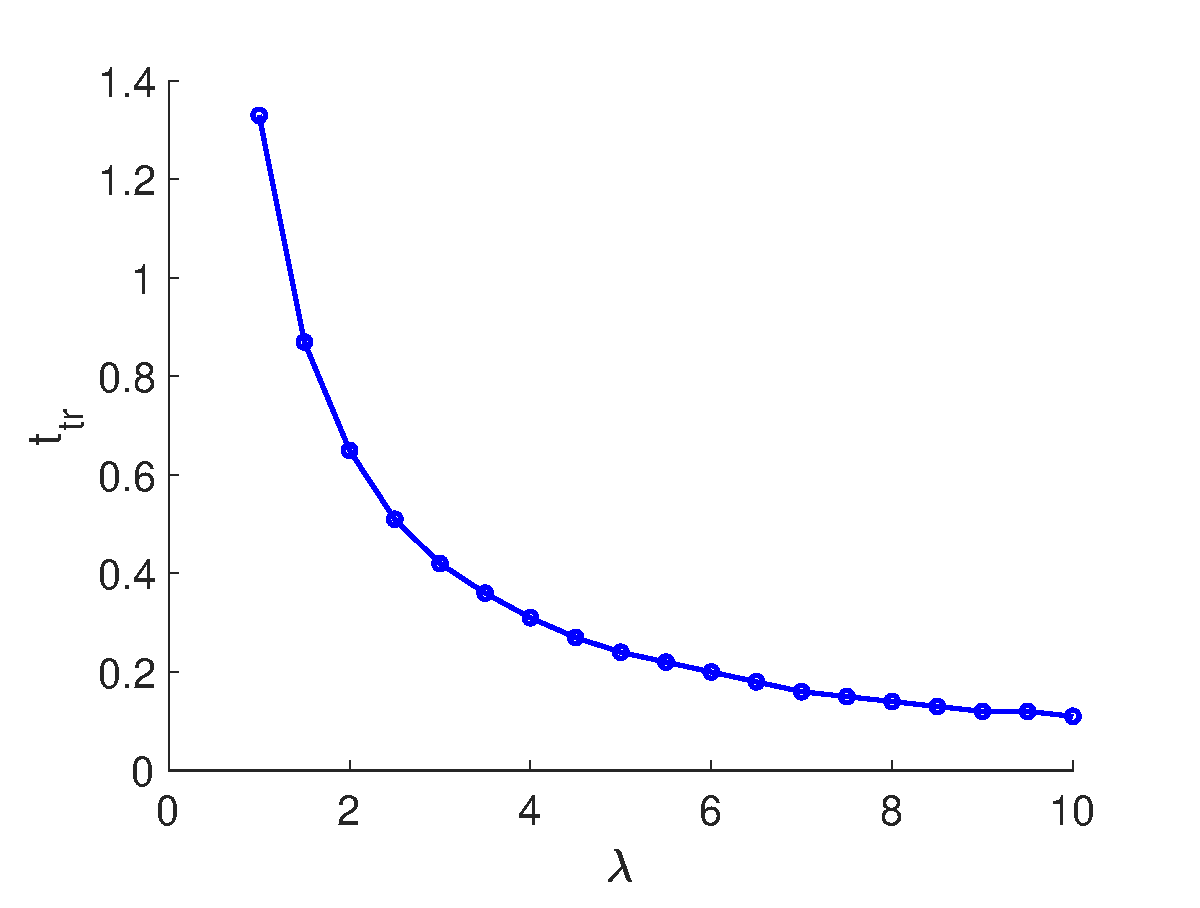
\includegraphics[width=1\linewidth]{Images/photo8_1.eps} 
  \end{minipage} 
  \begin{minipage}{0.45\linewidth}
  \centering
    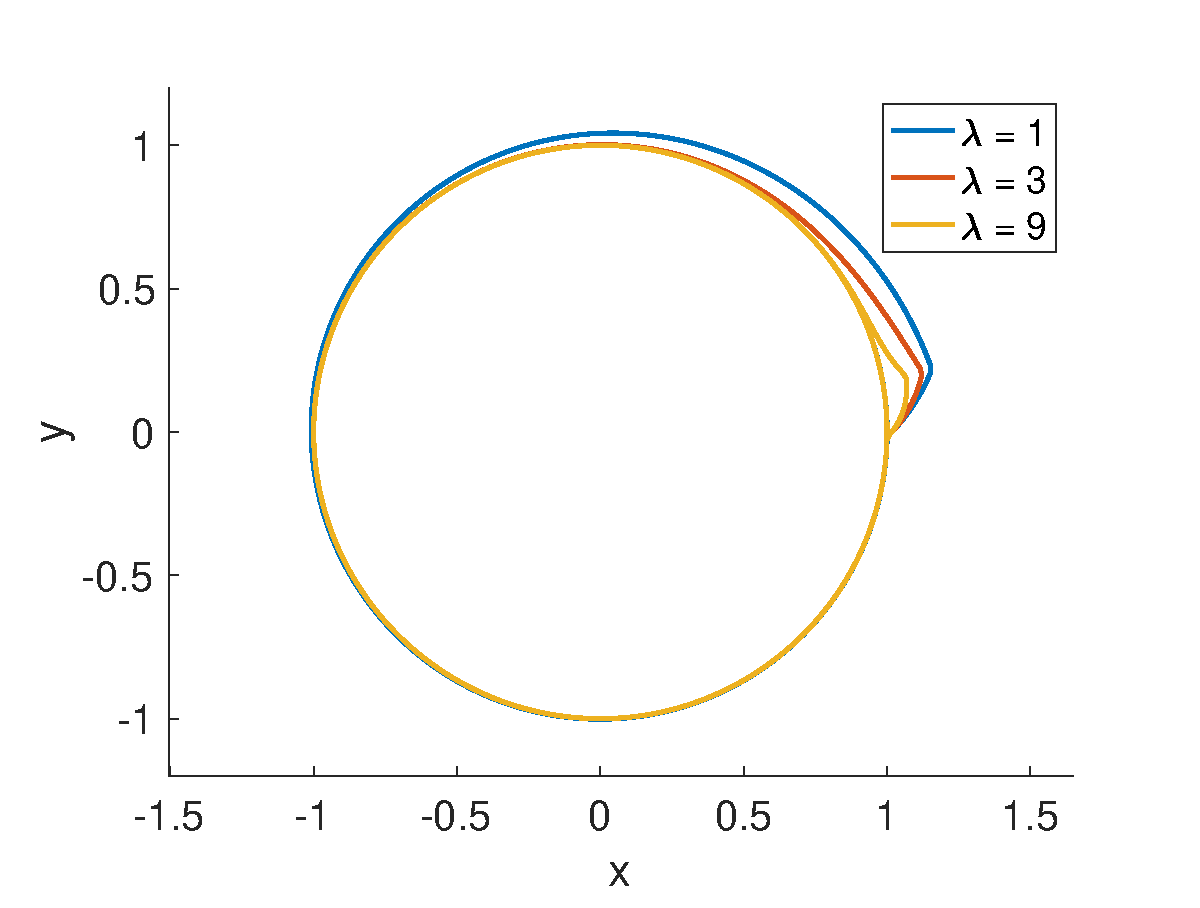
\includegraphics[width=1\linewidth]{Images/photo8_2.eps} 
  \end{minipage} 
  
  \caption{\textbf{Perturbed $\Lambda \Omega_{2}$ system within the same amplitude level set and recovery times.} Left: recovery times for different values of parameter $\lambda$ where $K_{a} = 1$. Right: perturbation shown on the $x-y$ parameter space for different values of parameter $\lambda$ where $K_{a}=1$ ($b=\lambda$). Parameter values: $a = 1$ and $\omega = 1$.}
  \label{photo8}
\end{figure}


\subsection{Total-degeneracy}
Throughout this work two attributes are considered to characterize oscillatory solutions: the amplitude and frequency. Thus, we say a level set is total-degenerated when both the amplitude and frequency are constant. If two or more systems (or networks) belong to the same total-degenerated level set, we say that systems (or networks) are total-degenerated.

As an example, total-degenerated level sets in $\Lambda \Omega_{2}$ systems preserving both the amplitude and frequency do exist and its analytical expression is given by Eqs. (\ref{e16}) and (\ref{e18}).

\section{Numerical Simulations}
All simulations have been performed and coded in MATLAB (Math Works, MA). The numerical simulations were computed by using the modified Euler method (Runge-Kutta, order two), with time steps within the $\Delta t =0.01$ and $\Delta t = 0.001$ range.
